\documentclass[
  printed, %% This option enables the default options for the
           %% digital version of a document. Replace with `printed`
           %% to enable the default options for the printed version
           %% of a document.
  twoside, %% This option enables double-sided typesetting. Use at
           %% least 120 g/m² paper to prevent show-through. Replace
           %% with `oneside` to use one-sided typesetting; use only
           %% if you don’t have access to a double-sided printer,
           %% or if one-sided typesetting is a formal requirement
           %% at your faculty.
  table,   %% This option causes the coloring of tables. Replace
           %% with `notable` to restore plain LaTeX tables.
  nolof,     %% This option prints the List of Figures. Replace with
           %% `nolof` to hide the List of Figures.
  nolot,     %% This option prints the List of Tables. Replace with
           %% `nolot` to hide the List of Tables.
  %% More options are listed in the user guide at
  %% <http://mirrors.ctan.org/macros/latex/contrib/fithesis/guide/mu/fi.pdf>.
]{fithesis3}
%% The following section sets up the locales used in the thesis.
\usepackage[resetfonts]{cmap} %% We need to load the T2A font encoding
\usepackage[T1,T2A]{fontenc}  %% to use the Cyrillic fonts with Russian texts.
\usepackage[
  main=english, %% By using `czech` or `slovak` as the main locale
                %% instead of `english`, you can typeset the thesis
                %% in either Czech or Slovak, respectively.
  english, german, russian, czech, slovak %% The additional keys allow
]{babel}
%% The following section sets up the metadata of the thesis.
\thesissetup{
    date          = \the\year/\the\month/\the\day,
    university    = mu,
    faculty       = fi,
    type          = bc,
    author        = Attila Zsíros,
    gender        = m,
    advisor       = Mgr. Jan Čejka,
    title         = {Using Kalman filters for pose estimation of mobile devices in simulated                     underwater environments},
    TeXtitle      = {Using Kalman filters for pose estimation of mobile devices in simulated                     underwater environments},
    keywords      = {Augmented reality, Extended Kalman filter, iMareCulture, Kalman filter,                     Motion tracking, Odometry, Pose estimation},
    TeXkeywords   = {Augmented reality, Kalman filter, Extended Kalman filter, iMareCulture,                     Motion tracking, Odometry, Pose estimation},
    abstract      = {This is the abstract of my thesis, which can

                     span multiple paragraphs.},
    thanks        = {These are the acknowledgements for my thesis, which can

                     span multiple paragraphs.},
    bib           = bibliography.bib,
}
\usepackage{makeidx}      %% The `makeidx` package contains
\makeindex                %% helper commands for index typesetting.
%% These additional packages are used within the document:
\usepackage{paralist} %% Compact list environments
\usepackage{amsmath}  %% Mathematics
\usepackage{amsthm}
\usepackage{amsfonts}
\usepackage{url}      %% Hyperlinks
\usepackage[textwidth=2.5cm]{todonotes}
\usepackage{markdown} %% Lightweight markup
\usepackage{listings} %% Source code highlighting
\lstset{
  basicstyle      = \ttfamily,%
  identifierstyle = \color{black},%
  keywordstyle    = \color{blue},%
  keywordstyle    = {[2]\color{cyan}},%
  keywordstyle    = {[3]\color{olive}},%
  stringstyle     = \color{teal},%
  commentstyle    = \itshape\color{magenta}}
\usepackage{floatrow} %% Putting captions above tables
\floatsetup[table]{capposition=top}
\begin{document}
\chapter*{Introduction}
    \addcontentsline{toc}{chapter}{Introduction}
    The seabed is often called the biggest museum in the world. Thousands of shipwrecks, ancient flooded cities, and other structures form our underwater cultural heritage. Because many of these objects are deprived of their context when exhibited on land, some sites offer \textit{in situ} experience, where scuba divers have the chance to experience them in their original surroundings \cite{unesco}. 

    Immersive technologies are extensively used at such archaeological sites since they can present information connected to user's location, e.g., historical facts, visual navigation, or even provide an augmented reality view of the original state of the structure. A European Union project, named iMareCulture\footnote{https://imareculture.eu/}, is concerned about developing such applications. One branch of the project, which this thesis is a part of, aims at implementing virtual visits in augmented reality.
    
    As defined in \cite{inertial_video}: ``Augmented reality (AR) systems supplement the real world with virtual (computer-generated) objects that appear to coexist seamlessly in the same space as the real world.'' A difficult task in AR is tracking, i.e., the real-time pose recovery from monocular video streams. Among other tracking methods \cite{fusion01}, there are two major ones that the thesis is dealing with:
    
    \begin{itemize}
      \item Vision-based methods provide high accuracy but slow update rates and require line-of-sight between the camera and the markers;
      \item Inertial tracking, performed by the sensors from the inertial sensor unit (IMU), provides high-frequency measurements but is unreliable to track position for long periods of time due to problems with sensor bias and drift.
    \end{itemize}
    
    The goal of this thesis is the fusion of these two complementary approaches to get more accurate pose estimations than by using any of them alone. It extends an existing prototype of a vision-based AR application for Android phones and tablets. The application uses methods from ArUco library\footnote{ArUco is an OpenSource library for camera pose estimation using squared markers. \url{https://www.uco.es/investiga/grupos/ava/node/26}} with 2D barcode markers, detected by the camera, that are to be distributed in the archaeological site. For sensor fusion, a common data fusion algorithm that combines and smooths the measured values - the Kalman filter - is utilized.
    
    The first chapter discusses the available AR platforms with references to related works. The next two chapters introduce the theoretical background of the tracking methods, the relations between the coordinate frames, and the Kalman filtering.
    
    The fourth chapter is about experiments. Firstly, it presents the technical equipment and testing conditions. Secondly, it shows the Kalman filter performance from more straightforward cases (only a single marker with accelerometer) to the complex ones, when all IMU sensors along with multiple markers are involved. Successively, motion tracking is used as ground-truth, and several non-linear variants, such as the Extended and Unscented Kalman filter, are built and compared to each other.
    
    In the last chapter, an upgraded working prototype of the AR application is tested in the Underwater Archaeological Park of Baia in Italy. The quality of the prototype is discussed, and gives suggestions for future development.

\chapter{Background}
    \begin{figure}
        \includegraphics[width=10cm]{img/Baia2.jpg}
        \caption{A tablet housed in a waterproof case showing an original reconstruction of Villa a Protiro.}
        \label{fig:baia2}
    \end{figure}

    The seabed is often called the biggest museum in the world. Throughout the history of human civilizations, entire cities have been flooded, and thousands of ships have sunken to the bottom of the lakes, seas, and oceans. In this subaqueous environment, they have been safely protected for thousands of years. Now they are a part of our cultural heritage in the same way as the heritage on land.
    
    Advances in technology have made the underwater world more accessible and therefore brought these sites within reach. The visitors are offered in situ experiences, which include dive trails, submersible tours for non-divers, and underwater museums \cite{unesco_online}.
    
    \textbf{Project iMare-Culture} focuses on promoting them to the wide public through the use of interactive technologies, virtual reality (VR), augmented reality (AR), and serious games\footnote{A serious game is a game designed for a primary purpose other than pure entertainment.}; all designed by scientists, researchers, archaeologists, and museum experts coming from eight Mediterranean countries.
    
    This thesis is a part of augmented reality research for this project. Figure \ref{fig:baia2} shows an example of AR usage, where the scuba diver is holding a tablet housed in a waterproof case, and observing an original reconstruction of Villa a Protiro in the Archaeological Underwater Park of Baia, Italy.

\chapter{Pose estimation for Augmented Reality}
    As Azuma defined in 1997, AR systems supplement the real world with virtual (computer-generated) objects that appear to coexist seamlessly with the real world. Besides aligning real and virtual objects with each other, these systems have to be interactive and in real time \cite{97azuma}. In contrast with VR, where the user is immersed in a virtual environment, AR allows interaction with virtual objects in a seamless way.

    The main AR research topics are Tracking Techniques, Interaction Techniques, Calibration and Registration, AR Applications, and Display Techniques \cite{17ISMAR}. Tracking is the most popular and fundamental one to deliver a coherent AR system. Its goal is to estimate the pose of the camera, i.e., the position and orientation relative to a reference frame. Despite the enormous progress in this field in the last ten years, it is still challenging to achieve low latency tracking with high precision, accuracy, jitter, and lag in a mobile device. If we compare AR and VR again, but now in terms of tracking requirements, AR is more demanding because errors in registration are easier to detect by the user \cite{93Azuma}.
    
    The tracking problem gets even more complex in underwater environments, where the system has to be waterproof, has to withstand the high pressure of diving depth, cannot rely on GPS, and the captured images suffer from turbidity effects caused by the medium.
    
    Furthermore, the amount and cost of sensors packed in smartphones are much more limited than in specialized devices used in for example robotics \cite{vi-sensor}. As a consequence, the measurements are noisier and biased. Tracking techniques tackle these problems by integrating several sensors with complementary characteristics into a sensor fusion filter. This chapter provides an overview of the pose estimation techniques and their utilization under water.

    \section{Tracking techniques}
        \subsection{Visual tracking}
            Vision-based techniques use computer vision methods to calculate the camera pose relative to real-world objects \cite{99SoYou,02Pinz}. They provide high accuracy over a large workspace, low jitter, and no drift. The frames are grabbed at rates of 30-60Hz. The general drawbacks include that they require line-of-sight between the camera and the detected target, and that motion blur in the image during drastic motions leads to temporary loss of real-time tracking abilities. The targets of the detector are either markers (marker-based tracking) or distinctive features in the image (markerless tracking). 
    
            Marker-based tracking methods simplify the problem of detecting 3D objects by detecting only 2D artificial markers that are easy to recognize \cite{19Cejka}. The most dominant technique in marker-based tracking is detecting square markers. They are easy and fast to detect and contain enough information to compute their relative pose to the camera. Examples of some software libraries are ARToolKit \cite{ARToolKit}, ARTag \cite{ARTag}, ARUco \cite{ARUco}, AprilTag \cite{AprilTag}. Besides square markers, other types of markers are also used in AR. For example circular or elliptic markers \cite{CircularMarker, EllipticMarker}. The elliptic shape of their contours provides more information about the position than in the case of square markers. Thus, they can be detected even when they are partially occluded. This is, however, paid by higher processing time. Other types of markers are described in \cite{OtherMarker1, OtherMarker2, OtherMarker3, OtherMarker4, OtherMarker5}.
            
            Instead of detecting artificial markers, markerless tracking methods detect the distinctive features in the image like edges, corners, or textures. The detection algorithms consist of two parts: detection of these features and computation of a descriptor for each feature that can match the features between frames \cite{19Cejka}. The speed and accuracy depend on the complexity of the scene. While simple targets like blobs or corners can be easily identified, cluttered scenes with many objects which are moving independently are extremely difficult to handle \cite{02Pinz}. This method is also not suitable for textureless environments. Examples of algorithms for natural feature detection used in augmented reality are SIFT \cite{SIFT}, SURF detector \cite{SURF}, and FAST \cite{FAST}. Markerless tracking is further used in simultaneous localization and mapping (SLAM) solutions described later in this chapter.
        
            \begin{figure}
                \includegraphics[width=10cm]{example-image}
                \caption{Different types of markers}
                \label{fig:Markers}
            \end{figure}
            
            Under-water localization from vision is still an open problem, and the state-of-the-art algorithms in visual odometry or SLAM do not give satisfying results \cite{17Weidner}. Most of the difficulties arise due to visual degradations caused by the medium. First, the strong light absorption shortens the visual perception to a few meters and makes the presence of an artificial lighting system mandatory when operating in deep waters. Second, the propagation of light is scattered by floating particles, causing turbidity effects on the captured images. Finally, the artificial light attracts the animals, and they tend to get in the field of view of the camera, which leads to occlusions in the images.
    
        \subsection{Inertial tracking}
            Most smartphones have an Inertial Measurement Unit (IMU) for monitoring the body's movement or orientation in three-dimensional space with respect to the Earth coordinate system. The IMU consists of a triple axis accelerometer and a triple axis gyroscope, see Figure \ref{fig:AndroidIMU}. The accelerometer senses the acceleration of the sensor along of each input axis, while the gyroscope measures the angular velocity around each input axis. Together, they form a 6 DoF (Degrees of Freedom) tracking system, i.e., tracking movement in 3 axes plus rotation in 3 axes (pitch, roll, yaw). Sometimes a third set of sensors, magnetometers, is added for heading reference (yaw axis), measuring the Earth's magnetic field. However, they are easily distorted by any nearby metallic substance that disturbs the magnetic field \cite{08ISMAR}. Thus, they are not further used in this thesis.
            
            \begin{figure}
                \includegraphics[width=6cm]{img/AndroidIMU.png}
                \caption{Coordinate system (relative to a device) that's used by the Android Sensor API.\protect\footnotemark}
                \label{fig:AndroidIMU}
            \end{figure}
            \footnotetext{\url{https://developer.android.com/guide/topics/sensors}}
            
            \subsubsection{MEMS}
            As opposed to the traditional mechanical IMUs, the IMUs in smartphones are based on MEMS (Microelectromechanical systems) technology. On the one hand, this makes them lightweight, compact, power-efficient, and less expensive, thus well suited for mobile computing. On the other hand, due to imperfections of the manufacturing and physical characteristics of the sensors, real IMU measurements are usually affected by random noise and systematic errors, such as bias, inaccurate scale factors, axis misalignments, and g-sensitivity \cite{19Xiao, 94Titteron, 03Nassar}. These errors may significantly influence the performance of visual-inertial methods.
            
            The following example illustrates these errors on the accelerometer: The accelerometer measures proper accelerations that are accelerations relative to a free fall. For example, if the device is laying flat on the table, the accelerometer should measure an acceleration of $1g \approx 9.81 m/s^2$ away from the center of the Earth. In contrast, when the device is in free fall, it should measure zero. However, as shown in Figure \ref{fig:imu_errors}, due to the bias of $-0.06 m/s^2$ and random noise of $0.02 m/s^2$, the measured acceleration is $9.77 m/s^2$.

            \begin{figure}
                \includegraphics[width=10cm]{img/IMU_errors.png}
                \caption{The bias (the offset of the sensor measurement from the physical input), noise (or gain is the random noise that affects the sensor measurements), and the scale factor (the relation between input and output) \cite{novatel}.}
                \label{fig:imu_errors}
            \end{figure}
            
            Thus, the sensor measurements are modeled as follows:
            \begin{align} 
                a_m &= (a - g) + b_a + n_a \\
                w_m &= w + b_\omega + n_\omega
            \end{align}
            where $a_m$ and $w_m$ are the raw measurements of accelerometer and gyroscope, respectively, $a$ and $w$ are linear acceleration and angular velocity of the body frame. $g$ is the gravity vector, $b_a$ and $b_\omega$ are the accelerometer and gyroscope biases respectively, $n_a$ and $n_\omega$ are the measurement noises. In this thesis, $n_a$ and $n_\omega$ are assumed to be Gaussian white noise, $n_a \sim \mathcal{N}(0,\sigma^2_a), n_\omega \sim \mathcal{N}(0,\sigma^2_\omega)$. For other IMU measurement models involving scale factors, axis misalignment, g-sensitivity, etc., please refer to \cite{16Rehder}. Calibration techniques are used to obtain the value of the bias.
            
            \subsubsection{IMU Calibration}
            To identify the value of bias and other intrinsic parameters of sensors for compensating the measurement errors, we use IMU calibration \cite{19Xiao}. Calibration is done by comparing the raw measurements to some known reference values and minimizing the differences between them. The reference calibration values can be estimated offline or online. 

            Offline calibration is relevant in the case of high-performance sensors which are manufactured precisely or factory calibrated carefully, and each sensor is sold with its own calibration parameters stored into the firmware \cite{14Tedaldi}. However, in consumer electronics, low-cost IMUs are used. The traditional high precision calibration methods require special external equipment such as motion tracking system \cite{04Kim}, which is often time-consuming and more expensive than the IMU itself. Moreover, the intrinsic calibration parameters may vary with mechanical shocks, temperature, and other factors. Treating these parameters as a constant would lead to performance degradation of the inertial tracking system \cite{19Xiao}. For an example of offline accelerometer calibration, please refer to \cite{98Lotters}.
            
            In contrast, online calibration is repeating the calibration process periodically. It is performed real time and without any external equipment. For example, Xiao et al. \cite{19Xiao} used this method to concurrently perform 3D pose estimation and online IMU calibration based on optimization methods in unknown environments without any external equipment. This thesis also utilizes the online calibration method.
            
            \subsubsection{Other IMU drawbacks}
            Besides bias and gain, another issue arises when using IMUs for navigation is the drift, an ever-increasing difference between where the system thinks it is located and the actual location. The drift occurs due to integrations with respect to time, where even small errors in measurements accumulate over time. In the case of position, the first integration of acceleration returns velocity and the second returns position. A constant error in acceleration results in a linear error in velocity and a quadratic error growth in the position \cite{08Springer}.

            If the angular velocity measurements from the gyroscope are integrated to obtain the orientation, the errors accumulate over time similarly to the accelerometer. Thus, in many attitude estimation solutions, the two sensors are fused because of their complementary characteristics: the gyroscope is accurate for quick movement in short periods of time, and the accelerometer determining the gravitation vector in longer periods of time \cite{99Luinge}. Fusing gyroscopes and accelerometers allows determining pitch and roll axes.
            
        \subsection{Hybrid tracking}
        Hybrid tracking is a promising alternative to tracking techniques. It combines multiple sensors to build more robust and accurate tracking systems. This sensor fusion exhibits the virtues of both technologies and compensates for their respective drawbacks \cite{99SoYou}.

        Visual-inertial tracking takes advantage of the complementary properties of visual and inertial sensors \cite{16Palonen}. On the one hand, the drawbacks of vision tracking, i.e., low-frequency, line-of-sight requirement, and slow motions due to motion blur, are compensated by the advantages of the IMU, i.e., high-frequency measurements from the IMU, occlusion immunity, and high accuracy in cases of rapid directional changes or high rotational speed. On the other hand, the inertial navigation systems are not accurate in slow rotational and translational motions due to bias and drift which is compensated by the high accuracy of the optical tracking system.
        
        Several approaches are tackling the visual-inertial estimation problem. Leutenegger \cite{15Leutenegger} separates them in two ways. First, the methods can be divided into batch nonlinear optimization methods and recursive filtering methods. Second, the two other categories of approaches found in the literature are described in \cite{15Leutenegger} as follows:
        \begin{itemize}
            \item loosely coupled systems - they independently estimate the pose by a vision-only algorithm and fuse IMU measurements only in a separate estimation step, limiting computational complexity;
            \item tightly coupled approaches - they, in contrast, include both the measurements from the IMU and the camera into a common problem where all states are jointly estimated, thus considering all correlations amongst them.
        \end{itemize}
        This thesis uses recursive filtering by utilizing the extended Kalman filter, and the tightly coupled approach, which proved to be essential for any high-precision visual-inertial navigation system and is implemented in most high-accuracy visual-inertial systems estimators \cite{13Leutenegger}.
        
        \subsection{SLAM}
        Hybrid tracking approaches are often combined with simultaneous localization and mapping (SLAM). SLAM is the computational problem of building a map of an unknown environment and, at the same time, using this map to compute the pose of the tracking device \cite{SLAMII}. It is a markerless technology, i.e., no markers or image targets are necessary to place in the environment. The map is created by obtaining spatial data of the environment, for example, 3D point clouds. Mapping and tracking simultaneously have high computational demands on the device, which is also a reason why SLAM solutions were initially employed in systems with specialized equipment, for example in robotics, self-driving cars, or unmanned aerial vehicles. However, thanks to advances in computer vision, performance, and sensory navigation of mobile devices in the past decade, smartphones are powerful enough to run AR applications that use SLAM. For general concepts of existing mobile SLAM techniques, please refer to \cite{17Taketomi} and for a survey of 23 chosen methods to \cite{16Younes}.

        Since there is no need for adding other elements in the environment and today's smartphones have enough computing power, many commercial AR software development kits (SDK) are based on SLAM. The most powerful and popular SDK's are ARCore (Google) \cite{ARcore}, ARKit (Apple) \cite{ARkit}, and Vuforia (PTC) \cite{Vuforia}. They offer native application programming interfaces (API's) for motion tracking, environmental understanding, and light estimation to simplify the task of building an AR experience. The developer can make use of the detection of horizontal surfaces, point cloud anchors, and virtual objects lighting that matches the surroundings to make their appearance more realistic. Amin and Govilkar give a comparative study of AR SDK's in \cite{Comparative}.
        
    \section{Underwater pose estimation}
    \label{sec:underwater_pose_estimation}
    Under the water, the number of requirements for an AR system is higher than on land. The system has to be waterproof, has to withstand the high pressure of diving depth and cannot rely on GPS \cite{18Ferrera}. This leads to the use of expensive, robust systems (e.g., remotely operated vehicles (ROVs) or autonomous underwater vehicles (AUVs)) that have to be equipped with advanced sensors (e.g., sonars, acoustic positioning systems, or Doppler velocity loggers (DVLs)), which are not suitable for mobile AR.

    Some solutions found in the literature rely on IMUs, pressure sensors and DVLs \cite{14Paull}, which, as discussed in this chapter, leads to unavoidable drift over time due to measurement noise. The drift is constrained using complementary sensors such as cameras or acoustic positioning systems. However, at close-range, acoustic systems do not provide accurate enough localization information whereas visual sensing can be highly effective \cite{18Palomeras}. Nevertheless, as discussed in the introduction of this chapter, the captured images are degraded by turbidity. Furthermore, the information delivered by sonar is not as rich as optical images \cite{15BoninFont} and remain very challenging to analyze.
    
\chapter{Kalman filtering}

\chapter{Localization in a simulated underwater environment}
The goal of this thesis is to choose a mobile, fiducial based, visual-inertial pose tracking system, and to evaluate its performance in underwater conditions. To be able to assess the tracking precision, the pose estimates have to be compared to ground truth. 

For position and orientation tracking, ground truth is typically represented by an external motion capture system with submillimeter accuracy \cite{15Neunert}. However, this system can only be installed in a controlled environment of a laboratory and cannot be used in the sea. Thus, the experiments in this thesis are conducted in the laboratory equipped with a motion capture system, and the underwater conditions are simulated by post-
-processing marker detection results.

In this chapter, section \ref{sec:pose_system} introduces the chosen underwater localization method, section explains how the low visibility conditions are simulated, and Section 2.3 describes how the accuracy of the localization is evaluated.

\section{Pose estimation system}
\label{sec:pose_system}
When choosing a suitable solution for underwater localization in the context of this thesis, various constraints have to be taken into account. As discussed in \ref{sec:underwater_pose_estimation}, some sensors, for example, GPS or magnetometers, are not suitable for underwater use, which already discards a large number of implemented localization systems found in the literature. 
 
In addition, besides using square fiducial markers, the system should be completely self-contained, i.e., not relying on any external equipment often used under water \cite{14Paull}, such as acoustic positioning systems.


    \subsection{RCARS}
    Although we did not find any mobile pose tracking system customized for underwater use at the time of our related work research, we found a suitable open source solution from the field of robotics. 
    
    \textbf{RCARS} (Robot-Centric Absolute Reference System) is a fiducial-based, visual-inertial EKF-SLAM state estimation system,  introduced by Neunert et al. in 2016 \cite{15Neunert}. As the authors claim, coupling SLAM and fiducial based estimation resulted in a leaner estimation and smaller map sizes, which makes the system more lightweight. Moreover, they state that the system provides accurate estimates and is robust against fast motions and changing lighting conditions.

    \subsection{ROS}
    RCARS is built on the Robot Operating System\footnote{\url{https://www.ros.org/}} (ROS) software interface. ROS is an open-source, robotics middleware for creating robot applications. It provides services such as hardware abstraction, device drivers, libraries, visualizers, message-passing, and package management. 
    
    ROS-based processes are represented as \textit{nodes} in a graph architecture, connected by edges called \textit{topics}. Topics are buses over which nodes send and receive messages. To send a message, a node must \textit{publish} to a topic, while to receive messages it must \textit{subscribe}. The types of messages passed on a topic vary widely and can be user-defined. The content of these messages can be sensor data, motor control commands, state information, actuator commands, or anything else.
    
    \missingfigure[figwidth=10cm]{RCARS nodes}
    
    \subsection{RCARS packages}
    The RCARS the software structure\footnote{\url{https://bitbucket.org/adrlab/rcars/wiki/Software_Structure}}, generated by the \texttt{rqt\_graph} tool, is visualized in Fig. X. RCARS operates on three nodes --- the estimator, the detector, and the visualizer --- and the topics passed between them are, for example, the image (\texttt{/cam0/image\_raw}), the IMU measurements (\texttt{/imu0}), or the detected tags (\texttt{/rcars/detector/tags}).
    
    \missingfigure[figwidth=10cm]{RCARS visualizer}

    The detector detects markers in the received undistorted images and publishes marker information, such as the marker id, the marker pose with recpect to camera, or the locations of its four corners in the image coordinates. 
    
    RCARS uses AprilTags as markers, shown in Fig.X, which are 2-dimensional, square printable markers with a unique identification number. As a result, they can be robustly tracked and estimated in the EKF. As Neunert et al. reason, AprilTags are used in RCARS due to their high accuracy and the numerous available detector implementations in C/C++. They also state that with AprilTags, high accuracy tracking is achievable even with very few tags, resulting in lower computational demands.
    
    \missingfigure[figwidth=10cm]{AprilTag}

    The estimator realizes the Kalman filtering. It subscribes to the detected markers and the inertial measurements, and uses them for estimating the pose of the device, as well as the extrinsic calibration between the IMU and the camera. 
 
    The visualizer uses \texttt{rviz}\footnote{\url{http://wiki.ros.org/rviz}} for a 3D visualization of the workspace, as well as an image preview. As seen in Fig.X, the image preview shows both the tag corner detections (in blue) and their corresponding estimations (in red). This information is useful for analyzing the estimation process, particularly for identifying the cases when outliers occur.
    
    \section{Utilizing RCARS}
    The drawback of RCARS is that it runs only on a computer. Thus, the pose estimation cannot be realized online on the Android smartphone used in this thesis, which leads to a series of steps that need to be done to be taken in order to obtain the pose estimates from RCARS. This workflow is depicted in Fig.X
    
    \missingfigure[figwidth=10cm, figheight=10cm]{Workflow}
    
    \subsection{Input data}
    First, the measurements from the smartphone have to be set as input for RCARS. ROS provides packages\footnote{\url{http://wiki.ros.org/rosserial}} for communication with the serial ports of electronic devices connected to the computer, allowing live sending of data to ROS; however, these packages are built mainly for microcontrollers such as Arduino. Although there is also a driver\footnote{\url{http://wiki.ros.org/android_sensors_driver}} for a  wireless communication with Android devices, it supports only sending GPS and IMU measurements, not the camera images that are needed here.

    Therefore, in our experiment, we first need to record the datasets and then convert the image and the IMU measurements to into a proper input format to allow sending them within the ROS ecosystem. 
    
    The recording is realized by the iMareCameraRecorder application developed by Jan Čejka for the AR systems research within the project iMareCulture. This application allows recording of uncompressed, time-stamped images and IMU measurements.

    To run RCARS on these measurements, they are saved into a \textit{bag}\footnote{\url{http://wiki.ros.org/Bags}} file as ROS \textit{messages}. The \textit{bag} is a file format for storing ROS message data. The conversion is realized by the \texttt{phone\_to\_bag.py} Python script that uses the \textit{rosbag} Python API\footnote{\url{http://wiki.ros.org/rosbag/Code\%20API\#py_api}} to write into a \textit{bag} file. The \textit{messages} are stored in this file in the following \textit{topics}:
    \begin{description}
        \item [\textbf{camera\_info}] holds the camera metadata, such as the intrinsic calibration parameters or the image resolution;
        \item [\textbf{image\_raw}] holds the raw camera images;
        \item [\textbf{imu}] holds the accelerometer and gyroscope measurements.
    \end{description}
	
    The script synchronizes the IMU with the images based on the their timestamps. Note that RCARS allows using only one sampling frequency for the IMU measurements. For example, in the case of the iMareCameraRecorder, even though it records the accelerometer at 400Hz and the gyroscope at 200Hz, the accelerometer had to be downsampled to 200Hz to match the frequency of the gyroscope. In addition, we use the \textit{rosbag}\footnote{\url{http://wiki.ros.org/rosbag}} tools for recording and playing back bag files.

    When the bag files are prepared, we play them with rosbag. When the bag file is being played, it appears to RCARS as if there was a live stream of data from a device, which finally allows us to RCARS on our data.
    
    \subsection{Detection}
    First, as shown in our workflow in Fig.X, the integrated ROS image processing node\footnote{\url{http://wiki.ros.org/image_proc}} undistorts the raw image using the intrinsic camera calibration parameters in the \texttt{camera\_info} topic.

    \subsection{Estimation}
    Second, these undistorted images, as well as the IMU measurements, proceed to the estimator node. The estimator provides a configuration file \texttt{EKFSettings.info}\footnote{\url{https://bitbucket.org/adrlab/rcars/wiki/Configuration}} that allows customizing the EKF parameters to our device. Since configuring an EKF is not trivial and requires some experience, we left most of the parameters on default. 
    
    However, since the device Neunert et al. \cite{15Neunert} use is the specialized Visual-Inertial (VI-) Sensor\footnote{\url{http://wiki.ros.org/vi_sensor/}}, there are parameters that have to be changed because we are using a different device:
    \begin{enumerate}
        \item the extrinsic calibration between the IMU and the camera;
        \item the squared pixel standard deviation of the tag corner detection results;
        \item and the Mahalonobis threshold defining when a marker is considered an outlier.
    \end{enumerate}
	
    Enough time should be devoted to determining these values for the device, because they are critical for the estimator to work correctly. Also note that the VI-Sensor,  provides fully time-synchronized and factory calibrated IMU- and stereo-camera data stream. Therefore, we do not expect from the smartphone to perform in our experiments with such accuracy and robustness as the authors achieved.
    
    The estimator then finally publishes the pose estimates of the device (\texttt{filterPose} topic) and all tags (\texttt{tagsInertialFrame} topic) in the filter frame. 
    
    The coordinate frames used in RCARS can be identified in \textit{rviz} that provides a 3D visualization of the workspace. As shown in Fig.X, the estimator works with different coordinate systems for the workspace, IMU, camera, and each tag. The origin of the workspace frame is set at the time of the estimator initialization, i.e., when it starts receiving the smartphone measurements. This frame assumes that the gravity points in negative z-direction.
    
    \missingfigure[figwidth=10cm]{Coordinate frames}
    
    We then record the topics from the estimator that we are interested in again into a bag file. Consequently, this bag is converted into the csv\footnote{\url{https://en.wikipedia.org/wiki/Comma-separated_values}} format, which is analyzed in MATLAB in the evaluation section, see \ref{sec:evaluation}.

\section{Simulating underwater environments}
This thesis aims at evaluating decreased visibility conditions of underwater environments. In marine terms, visibility is an estimation of water clarity and is defined as the distance a diver can see horizontally \cite{visibility}. There are several factors affecting the visibility; for example, light attenuation and scattering between the object and the viewer result in lower contrast and blur in the image. The visibility can also be severely decreased by suspended particles of sand, mud, clay, or other bottom sediments.

However, these conditions are difficult to imitate in the laboratory. Thus, we record the datasets in full visibility and then modify the detection results by adding several steps in our pose estimation workflow. This section describes the two underwater conditions simulated in this thesis: short-range visibility (\ref{sec:threshold}) and water turbidity (\ref{sec:noise}).

    \subsection{Distance threshold}
    \label{sec:threshold}
    This simulation assumes that after a certain distance threshold, no markers are visible in the image. We realize this as follows.
    
    First, the detector detects all tags in the raw image, which corresponds to the full visibility conditions and serves as a reference for comparison in the evaluation section. The detection results are then saved in a bag file named \textttt{<dataset>\_tags.bag}.
    
    Second, the Python script \textttt{threshold.py} takes this bag file and discards the markers further away from the camera than a given threshold. This is achieved by comparing the threshold to the z-coordinate of the marker pose relative to the camera. We also consider a linear falloff distance of one meter for discarding the markers. FigX shows an example with a threshold of 3 meters, where tags closer to the camera than 2 meters remain in the bag, tags at 2.5 meters have a 50 \% chance of being discarded, and all tags 3 or more meters far are discarded.
    
    \begin{figure}
        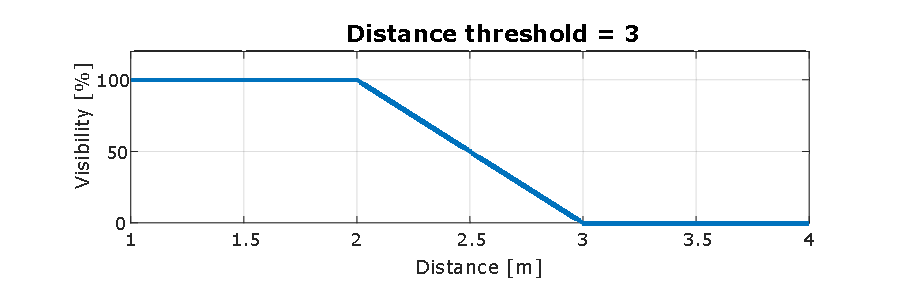
\includegraphics[width=12cm]{img/falloff.eps}
        \caption{Falloff}
        \label{fig:falloff}
    \end{figure}
    
    Finally, the threshold.py script outputs a bag file named \\ \textttt{<dataset>\_<threshold>\_tags.bag}, which is then sent to the estimator that outputs the pose estimates in low visibility into a bag file named \texttt{<dataset>\_<threshold>\_est.bag}.
    
    \subsection{Adding noise}
    \label{sec:noise}
    The second simulation assumes that there are floating particles in the water that bring noise into tag corner detection. We simulate this by corrupting the tag corner detections by random noise of a given variance. We are using the fact that the EKF in RCARS uses the tag corner detections as observations rather than the tag pose obtained by OpenCV. As a result of this holistic approach, we can improve the tracking by changing the PixelStd parameter in the EKFSettings.info file. The PixelStd parameter represents the pixel variance (the squared pixel standard deviation) of the tag corner detections.
    
    In full visibility, we use a pixel variance of 25 pixels. After adding noise to the corners, we raise this variance accordingly. For example, for noise with variance of 100 pixels, we set the "PixelStd" parameter to 125.
    
    The workflow is similar to the thresholding. First, we obtain the \textttt{<dataset>\_tags.bag} file with full visibility from the detector. Second, the \textttt{add\_noise.py} script adds random noise with Gaussian distribution with zero mean and a given standard deviation. It uses the pseudo-random number generators Python module random\footnote{\url{https://docs.python.org/2/library/random.html}} with a seed 250. Finally, a file named \\ \textttt{<dataset>\_<standard\_deviation>px\_<PixelStd\_parameter\_value>\_tags.bag} is output, which is then processed by the estimator to obtain the pose estimates in the file \\
    \textttt{<dataset>\_<standard\_deviation>px\_<PixelStd\_parameter\_value>\_est.bag}.



\section{Evaluation method}
\label{sec:evaluation}

\chapter{Experiment}
\section{Setup}
Calibration and bias free comparison is essential for our experiment. This section describes the specific setup and conditions that our experiments were performed in.

    \subsection{Laboratory}
    The experiments took place at the Human-Computer Interaction laboratory\footnote{\url{http://hci.fi.muni.cz/}} at the Faculty of Informatics, Masaryk University in Brno. As shown in Fig. \ref{fig:hcil}, the markers were randomly placed across the room, covering an area of 5.4 x 6.6 meters; with the markers attached both on horizontal and vertical surfaces.
    
    \begin{figure}
        \includegraphics[width=8cm]{example-image}
        \caption{HCIL}
        \label{fig:hcil}
    \end{figure}
    
    The laboratory is equipped with a high-quality motion capture system from Optitrack\footnote{\url{https://optitrack.com/products/prime-13w/}} that uses 16 ultra-wide cameras (Prime13W), offering high-precision and low-latency tracking with up to 240 FPS capture rate. Tracking of an object is realized by spherical retroreflective markers detected by the cameras. This system is controlled by Motive software, which provides calibration, creating rigid bodies, and recording.
    
    Before recording the datasets, a new calibration was performed following the documentation\footnote{\url{https://v20.wiki.optitrack.com/index.php?title=Calibration}}, with exceptional results with the mean 3D error of 0.673 mm. In our experiments, the average error per marker was 0.1mm for the static marker, and 0.4mm for the moving smartphone.

    \subsection{Markers}
    \begin{itemize}
        \item apriltags
        \item in EKFsettings.info, number of dynamic tags is set to 30. I used 27 AprilTags downloaded from here: \url{https://robot2016.mit.edu/sites/default/files/documents/project_apriltag36h11.pdf}
        \item placed on flat surfaces or attached with pritt gum, or just loosely on a chair, being careful not to bend them
    \end{itemize}
    
    \subsection{Phone}
    The smartphone we used is the OnePlus 6 running on Android 9 and equipped with a 16 MP, f/1.7, wide-angle camera (25mm (wide), 1/2.6") and the BMI160\footnote{\url{https://www.bosch-sensortec.com/bst/products/all_products/bmi160}} IMU manufactured by Bosch Sensortec\footnote{\url{https://www.bosch-sensortec.com/}}.
    
    \subsection{Intrinsic calibration}
    The intrinsic camera calibration was performed in the laboratory to assert equal lighting conditions than in the datasets recordings. We used the OpenCV algorithm\footnote{\url{https://docs.opencv.org/2.4/modules/calib3d/doc/camera_calibration_and_3d_reconstruction.html}} that calculates both the camera matrix and the radial and tangential distortion coefficients from a chessboard pattern. 
    We used a chessboard pattern with the count of inner corners along both sides of 9 x 6 and printed it on an A4 paper. The dimensions of one chessboard square were 25 x 25mm. The pattern, as well as the calibration images and coefficients, are provided in the attachments. 
    The calibration images were following the Matlab camera calibration workflow\footnote{\url{https://www.mathworks.com/help/vision/ug/single-camera-calibrator-app.html}}. As it says, to achieve a good camera calibration, between 10 and 20 images of the checkerboard pattern should be used. In addition, the images should be captured at a distance roughly equal to the distance from the camera to the objects of interest, without using autofocus or changing the zoom settings between images. Furthermore, since lens distortion increases radially from the center of the image and sometimes is not uniform across the image frame, the images should be taken at different orientations relative to the camera and the pattern must appear close to the edges of the captured images.

    \subsection{Extrinsic calibration}
    Due to the extrinsic calibration, we have to know where the IMU is located in the device. We tried to figure out this location from the OnePlus 6 motherboard photos. Although it indicated possible locations, the exact one was not clear. 
    Therefore, we used the online extrinsic calibration provided by RCARS. The calibration process, described in chapter X, returned the relative transformation estimate depicted in Fig. \ref{fig:extrinsic}. 

    \begin{figure}
        \includegraphics[width=8cm]{example-image}
        \caption{Extrinsic calibration - IMU 50cm in front of the camera}
        \label{fig:extrinsic}
    \end{figure}
    
    However, note that this estimate is still an approximation and may not reflect the true IMU location, thus the results may be affected by this error.
    
    \subsection{Phone rig}
    To track the phone pose with the motion capture system, we mount retroreflective markers tracked by the cameras on the phone. Thus, we built a custom rig from skewers and rubber bands, shown in FigX. Following the marker placement recommendations from the documentation\footnote{\url{https://v20.wiki.optitrack.com/index.php?title=Rigid_Body_Tracking}}, we attach five spherical markers on the skewer edges asymmetrically, to avoid congruency. 
    When a rigid body of this rig is created in Motive, its pivot point is at its geometric center. Thus, to put the pivot point to camera location, we measure the distance of the camera lens from the geometric center and translate the pivot point in Motive accordingly.
    
    \begin{figure}
        \includegraphics[width=8cm]{example-image}
        \caption{Phone rig}
        \label{fig:rig}
    \end{figure}

    This phone rig proved to be robust enough against deflection and, with the proper holding of the device, the rig is trackable by the motion capture system throughout the whole dataset with minimal detection losses.
    
    \subsection{Motion capture to filter estimation}
    As proposed in chapterX, the poses have to be aligned according to a common origin to be able to compare the poses measured by the motion capture and the filter. In this case, the origin is set to be the AprilTag with id 1.
    For position, we tackle the alignment as follows. The tag frame origin of the detected tag in OpenCV is in its geometrical center. Also, when a rigid body is created in Motive, its pivot point is placed at its geometric center. Thus, for tracking of the tag with motion capture, the reflective markers are placed onto the four corners of the tag, and a rigid body is created consequently. This way, we ensure that the origin of the marker pose is the same for both RCARS and motion capture.
    To be able also to compare the orientation of the mocap and the filter, we take the orientation in the filter as a reference. When OpenCV detects the tag, the tag is assigned orientation axes as shown in Fig.X. The axes of the camera are aligned with the tag when the phone is laying flat on the tag with the camera on top. Thus, initializing the axes for the tag and the phone, in the same way, allows us to also compare the orientation of the mocap measurements and the filter estimates.
    
    \begin{figure}
        \includegraphics[width=8cm]{example-image}
        \caption{Axes}
        \label{fig:axes}
    \end{figure}

    Since a new rigid body in motive has its axes aligned with the global coordinate axis, we place the tag aligned with the global frame. Then we lay the phone on the tag so that their geometrical centers overlap, as shown in FigX. Now the new rigid bodies for the tag and the phone can be created.
    
    \subsection{Recording}
    For recording the datasets on the smartphone, we used iMareCameraRecorder, developed by Jan Čejka. A recording contains accelerometer, gyroscope, and magnetometer measurements, and camera images with their corresponding timestamps. Note that the camera frames and the IMU samples are not synchronized as in the case of the specialized VI-Sensor, which may negatively affect the performance of the estimator.
    
    The application contains a configuration file for setting the image resolution and sampling rates. In the experiments, we used 1280x720 resolution, 30 frames per second, and the IMU sampling frequencies of 200Hz for gyroscope and 400Hz for the accelerometer. However, due to RCARS input requirements, we downsample the accelerometer to match the gyroscope frequency.

	
	\subsection{Computer}
	For running RCARS for estimation and MATLAB for evaluation, we primarily use the Lenovo Z580 laptop with Intel Core i7-3612QM 2.10GHz CPU and 8 GB of RAM.  In addition, for faster processing, we use a PC in the HCI laboratory with Intel(R) Core(TM) i7-8700 3.20GHz CPU and 32 GB of RAM.
	
	\subsection{RCARS}
	To run RCARS, we downloaded a Ubuntu 14.04 LTS virtual machine accessible on Nootrix.com\footnote{\url{https://nootrix.com/diy-tutos/ros-indigo-virtual-machine/}}, which has already preinstalled ROS Indigo and ROS tools. We tried to run it on the newest Ubuntu 18.04 first, however, we had dependency issues and failed to do so, similarly to other users discussing on Bitbucket\footnote{\url{https://bitbucket.org/adrlab/rcars/issues/4/rcars_detector_node-cant-run}}. 
    In this virtual machine, we installed RCARS according to the instructions in the project's repository \footnote{\url{https://bitbucket.org/adrlab/rcars/wiki/Home}}.

\section{Datasets}
As discussed in chapterX, the underwater conditions are simulated in two ways: by discarding the detected tags according to their distance from the camera, and by adding noise to the detected tag corners. 

Each simulation is executed on three different datasets. In datasets 1\_cw and 2\_ccw, we walk slowly one time around the room clockwise and counter-clockwise, respectively; avoiding rapid changes in movement or orientation. Nevertheless, shake still occurs in the image due to walking. 

In contrast, dataset 3\_random contains random trajectory movement with several fast motions to test both the filter robustness and outlier recovery. This kind of incautions use occurs in unexperienced users not aware of the importance of minimizing motion blur and shake when using the device.

All of these datasets are available in the attachments of this thesis. Note that we were not always working with the full lengths of the datasets; therefore, the intervals are provided in the parameter file for each dataset.

FigX shows the error per sample for each dataset, which is 13 cm for 1\_cw, 21 cm for 2\_ccw, and 31cm for 3\_random. It seems quite a lot for an AR experience. The way the error occurs in the datasets differs. For example, while the error in 2\_ccw accumulates throughout the whole dataset, the error in 3\_random rapidly rises at a certain point due to a fast movement but then starts converging to its true position, which is disrupted by the subsequent outliers.

\section{Results}
\subsection{Distance threshold}
\subsection{Added noise}

\section{Future work}
        

\chapter{Conclusion}
This thesis analyzed the underwater challenges of AR systems that are based on hybrid pose tracking and use Kalman filters for sensor fusion. First, the most popular motion tracking techniques were covered, and the Kalman filtering technique was explained. Then a solution suitable for underwater AR that uses fiducial markers and inertial measurements fused by the extended Kalman filter was chosen. Since this thesis focuses on smartphones, but the adopted solution is built for robots and runs only offline on the computer, the measurements of the smartphone had to be converted into an appropriate input format.

Further, experiments in a laboratory equipped with high-quality motion capture system were designed and performed. They aimed at simulating poor visibility conditions by (1) discarding markers according to their distance from the camera and by (2) corrupting the detected corners by adding artificial noise to simulate water turbidity.

The results showed that a threshold distance for a good AR experience is around 2.3 meters. When the visibility is lower, the pose estimates start diverging quickly. However, it heavily depends on the marker placement density. In a dataset with the camera pointing rather straight than downwards, focusing on distant objects, the threshold was around 2.5 meters with the mean error per sample of 10 centimeters. On the other hand, in a dataset with the camera pointing more downwards, even 1.9 meters provided a satisfactory tracking accuracy with the mean error per sample of 20 centimeters. Another observation is that markers placed more than 4 meters away from the camera don't contribute a lot to the pose estimation and can be discarded to lower the filter state size and thus improve the estimation speed.

Adding noise and, at the same time, raising the pixel standard deviation parameter of the EKF did not result in reducing the pose estimate accuracy significantly, which underwrites the robustness of the filtering system. 

The primary takeaways from the experiments include that the accuracy of the results heavily depends on the camera intrinsic and extrinsic calibration. Enough time should be dedicated to finding out these parameters, otherwise, the results are going to be misleading. 

The tracking accuracy also depends on the camera movement, which should be slow, controlled, and with minimized shake and motion blur. Furthermore, the autofocus of the camera should be turned off to avoid "focus breathing."

Future work will concentrate on developing a self-contained pose tracking system designed for smartphones, considering the low-cost sensors, low power consumption, and computational complexity constraints. In addition, the detector could search not only for fiducial markers but also for image features to achieve better precision and lower the field preparation requirements.


\printbibliography[heading=bibintoc] %% Print the bibliography.
\end{document}